
\section{Examples for the Import of Contributions}

The content within the following sections is generated via RDFtex's import functionality. \textbf{Attention:} This example is only for benchmarking purposes. Each import is included twenty times. 


\subsection{Dataset Import}

% RDFtex Dataset Import Start
\begin{dataset}
SciERC~\cite{DBLP:conf/emnlp/LuanHOH18}\\
Available at: \url{https://paperswithcode.com/dataset/scierc}\\
Domain: Artificial Intelligence\\
Description: ``Our dataset (called SciERC) includes annotations for scientific entities, their relations, and coreference clusters for 500 scientific abstracts."~\cite{DBLP:conf/emnlp/LuanHOH18}
\label{dataset:scierc0}
\end{dataset}
% RDFtex Dataset Import End% RDFtex Dataset Import Start
\begin{dataset}
SciERC~\cite{DBLP:conf/emnlp/LuanHOH18}\\
Available at: \url{https://paperswithcode.com/dataset/scierc}\\
Domain: Artificial Intelligence\\
Description: ``Our dataset (called SciERC) includes annotations for scientific entities, their relations, and coreference clusters for 500 scientific abstracts."~\cite{DBLP:conf/emnlp/LuanHOH18}
\label{dataset:scierc1}
\end{dataset}
% RDFtex Dataset Import End% RDFtex Dataset Import Start
\begin{dataset}
SciERC~\cite{DBLP:conf/emnlp/LuanHOH18}\\
Available at: \url{https://paperswithcode.com/dataset/scierc}\\
Domain: Artificial Intelligence\\
Description: ``Our dataset (called SciERC) includes annotations for scientific entities, their relations, and coreference clusters for 500 scientific abstracts."~\cite{DBLP:conf/emnlp/LuanHOH18}
\label{dataset:scierc2}
\end{dataset}
% RDFtex Dataset Import End% RDFtex Dataset Import Start
\begin{dataset}
SciERC~\cite{DBLP:conf/emnlp/LuanHOH18}\\
Available at: \url{https://paperswithcode.com/dataset/scierc}\\
Domain: Artificial Intelligence\\
Description: ``Our dataset (called SciERC) includes annotations for scientific entities, their relations, and coreference clusters for 500 scientific abstracts."~\cite{DBLP:conf/emnlp/LuanHOH18}
\label{dataset:scierc3}
\end{dataset}
% RDFtex Dataset Import End% RDFtex Dataset Import Start
\begin{dataset}
SciERC~\cite{DBLP:conf/emnlp/LuanHOH18}\\
Available at: \url{https://paperswithcode.com/dataset/scierc}\\
Domain: Artificial Intelligence\\
Description: ``Our dataset (called SciERC) includes annotations for scientific entities, their relations, and coreference clusters for 500 scientific abstracts."~\cite{DBLP:conf/emnlp/LuanHOH18}
\label{dataset:scierc4}
\end{dataset}
% RDFtex Dataset Import End% RDFtex Dataset Import Start
\begin{dataset}
SciERC~\cite{DBLP:conf/emnlp/LuanHOH18}\\
Available at: \url{https://paperswithcode.com/dataset/scierc}\\
Domain: Artificial Intelligence\\
Description: ``Our dataset (called SciERC) includes annotations for scientific entities, their relations, and coreference clusters for 500 scientific abstracts."~\cite{DBLP:conf/emnlp/LuanHOH18}
\label{dataset:scierc5}
\end{dataset}
% RDFtex Dataset Import End% RDFtex Dataset Import Start
\begin{dataset}
SciERC~\cite{DBLP:conf/emnlp/LuanHOH18}\\
Available at: \url{https://paperswithcode.com/dataset/scierc}\\
Domain: Artificial Intelligence\\
Description: ``Our dataset (called SciERC) includes annotations for scientific entities, their relations, and coreference clusters for 500 scientific abstracts."~\cite{DBLP:conf/emnlp/LuanHOH18}
\label{dataset:scierc6}
\end{dataset}
% RDFtex Dataset Import End% RDFtex Dataset Import Start
\begin{dataset}
SciERC~\cite{DBLP:conf/emnlp/LuanHOH18}\\
Available at: \url{https://paperswithcode.com/dataset/scierc}\\
Domain: Artificial Intelligence\\
Description: ``Our dataset (called SciERC) includes annotations for scientific entities, their relations, and coreference clusters for 500 scientific abstracts."~\cite{DBLP:conf/emnlp/LuanHOH18}
\label{dataset:scierc7}
\end{dataset}
% RDFtex Dataset Import End% RDFtex Dataset Import Start
\begin{dataset}
SciERC~\cite{DBLP:conf/emnlp/LuanHOH18}\\
Available at: \url{https://paperswithcode.com/dataset/scierc}\\
Domain: Artificial Intelligence\\
Description: ``Our dataset (called SciERC) includes annotations for scientific entities, their relations, and coreference clusters for 500 scientific abstracts."~\cite{DBLP:conf/emnlp/LuanHOH18}
\label{dataset:scierc8}
\end{dataset}
% RDFtex Dataset Import End% RDFtex Dataset Import Start
\begin{dataset}
SciERC~\cite{DBLP:conf/emnlp/LuanHOH18}\\
Available at: \url{https://paperswithcode.com/dataset/scierc}\\
Domain: Artificial Intelligence\\
Description: ``Our dataset (called SciERC) includes annotations for scientific entities, their relations, and coreference clusters for 500 scientific abstracts."~\cite{DBLP:conf/emnlp/LuanHOH18}
\label{dataset:scierc9}
\end{dataset}
% RDFtex Dataset Import End% RDFtex Dataset Import Start
\begin{dataset}
SciERC~\cite{DBLP:conf/emnlp/LuanHOH18}\\
Available at: \url{https://paperswithcode.com/dataset/scierc}\\
Domain: Artificial Intelligence\\
Description: ``Our dataset (called SciERC) includes annotations for scientific entities, their relations, and coreference clusters for 500 scientific abstracts."~\cite{DBLP:conf/emnlp/LuanHOH18}
\label{dataset:scierc10}
\end{dataset}
% RDFtex Dataset Import End% RDFtex Dataset Import Start
\begin{dataset}
SciERC~\cite{DBLP:conf/emnlp/LuanHOH18}\\
Available at: \url{https://paperswithcode.com/dataset/scierc}\\
Domain: Artificial Intelligence\\
Description: ``Our dataset (called SciERC) includes annotations for scientific entities, their relations, and coreference clusters for 500 scientific abstracts."~\cite{DBLP:conf/emnlp/LuanHOH18}
\label{dataset:scierc11}
\end{dataset}
% RDFtex Dataset Import End% RDFtex Dataset Import Start
\begin{dataset}
SciERC~\cite{DBLP:conf/emnlp/LuanHOH18}\\
Available at: \url{https://paperswithcode.com/dataset/scierc}\\
Domain: Artificial Intelligence\\
Description: ``Our dataset (called SciERC) includes annotations for scientific entities, their relations, and coreference clusters for 500 scientific abstracts."~\cite{DBLP:conf/emnlp/LuanHOH18}
\label{dataset:scierc12}
\end{dataset}
% RDFtex Dataset Import End% RDFtex Dataset Import Start
\begin{dataset}
SciERC~\cite{DBLP:conf/emnlp/LuanHOH18}\\
Available at: \url{https://paperswithcode.com/dataset/scierc}\\
Domain: Artificial Intelligence\\
Description: ``Our dataset (called SciERC) includes annotations for scientific entities, their relations, and coreference clusters for 500 scientific abstracts."~\cite{DBLP:conf/emnlp/LuanHOH18}
\label{dataset:scierc13}
\end{dataset}
% RDFtex Dataset Import End% RDFtex Dataset Import Start
\begin{dataset}
SciERC~\cite{DBLP:conf/emnlp/LuanHOH18}\\
Available at: \url{https://paperswithcode.com/dataset/scierc}\\
Domain: Artificial Intelligence\\
Description: ``Our dataset (called SciERC) includes annotations for scientific entities, their relations, and coreference clusters for 500 scientific abstracts."~\cite{DBLP:conf/emnlp/LuanHOH18}
\label{dataset:scierc14}
\end{dataset}
% RDFtex Dataset Import End% RDFtex Dataset Import Start
\begin{dataset}
SciERC~\cite{DBLP:conf/emnlp/LuanHOH18}\\
Available at: \url{https://paperswithcode.com/dataset/scierc}\\
Domain: Artificial Intelligence\\
Description: ``Our dataset (called SciERC) includes annotations for scientific entities, their relations, and coreference clusters for 500 scientific abstracts."~\cite{DBLP:conf/emnlp/LuanHOH18}
\label{dataset:scierc15}
\end{dataset}
% RDFtex Dataset Import End% RDFtex Dataset Import Start
\begin{dataset}
SciERC~\cite{DBLP:conf/emnlp/LuanHOH18}\\
Available at: \url{https://paperswithcode.com/dataset/scierc}\\
Domain: Artificial Intelligence\\
Description: ``Our dataset (called SciERC) includes annotations for scientific entities, their relations, and coreference clusters for 500 scientific abstracts."~\cite{DBLP:conf/emnlp/LuanHOH18}
\label{dataset:scierc16}
\end{dataset}
% RDFtex Dataset Import End% RDFtex Dataset Import Start
\begin{dataset}
SciERC~\cite{DBLP:conf/emnlp/LuanHOH18}\\
Available at: \url{https://paperswithcode.com/dataset/scierc}\\
Domain: Artificial Intelligence\\
Description: ``Our dataset (called SciERC) includes annotations for scientific entities, their relations, and coreference clusters for 500 scientific abstracts."~\cite{DBLP:conf/emnlp/LuanHOH18}
\label{dataset:scierc17}
\end{dataset}
% RDFtex Dataset Import End% RDFtex Dataset Import Start
\begin{dataset}
SciERC~\cite{DBLP:conf/emnlp/LuanHOH18}\\
Available at: \url{https://paperswithcode.com/dataset/scierc}\\
Domain: Artificial Intelligence\\
Description: ``Our dataset (called SciERC) includes annotations for scientific entities, their relations, and coreference clusters for 500 scientific abstracts."~\cite{DBLP:conf/emnlp/LuanHOH18}
\label{dataset:scierc18}
\end{dataset}
% RDFtex Dataset Import End% RDFtex Dataset Import Start
\begin{dataset}
SciERC~\cite{DBLP:conf/emnlp/LuanHOH18}\\
Available at: \url{https://paperswithcode.com/dataset/scierc}\\
Domain: Artificial Intelligence\\
Description: ``Our dataset (called SciERC) includes annotations for scientific entities, their relations, and coreference clusters for 500 scientific abstracts."~\cite{DBLP:conf/emnlp/LuanHOH18}
\label{dataset:scierc19}
\end{dataset}
% RDFtex Dataset Import End
\Cref{dataset:scierc0} shows an imported dataset.

\subsection{Definition Import}

% RDFtex Definition Import Start
\begin{definition}
\label{def:knowledge-graph0}
A knowledge graph acquires and integrates information into an ontology and applies a reasoner to derive new knowledge.\normalfont{~\cite{DBLP:conf/i-semantics/EhrlingerW16}}
\end{definition}
% RDFtex Definition Import End% RDFtex Definition Import Start
\begin{definition}
\label{def:knowledge-graph1}
A knowledge graph acquires and integrates information into an ontology and applies a reasoner to derive new knowledge.\normalfont{~\cite{DBLP:conf/i-semantics/EhrlingerW16}}
\end{definition}
% RDFtex Definition Import End% RDFtex Definition Import Start
\begin{definition}
\label{def:knowledge-graph2}
A knowledge graph acquires and integrates information into an ontology and applies a reasoner to derive new knowledge.\normalfont{~\cite{DBLP:conf/i-semantics/EhrlingerW16}}
\end{definition}
% RDFtex Definition Import End% RDFtex Definition Import Start
\begin{definition}
\label{def:knowledge-graph3}
A knowledge graph acquires and integrates information into an ontology and applies a reasoner to derive new knowledge.\normalfont{~\cite{DBLP:conf/i-semantics/EhrlingerW16}}
\end{definition}
% RDFtex Definition Import End% RDFtex Definition Import Start
\begin{definition}
\label{def:knowledge-graph4}
A knowledge graph acquires and integrates information into an ontology and applies a reasoner to derive new knowledge.\normalfont{~\cite{DBLP:conf/i-semantics/EhrlingerW16}}
\end{definition}
% RDFtex Definition Import End% RDFtex Definition Import Start
\begin{definition}
\label{def:knowledge-graph5}
A knowledge graph acquires and integrates information into an ontology and applies a reasoner to derive new knowledge.\normalfont{~\cite{DBLP:conf/i-semantics/EhrlingerW16}}
\end{definition}
% RDFtex Definition Import End% RDFtex Definition Import Start
\begin{definition}
\label{def:knowledge-graph6}
A knowledge graph acquires and integrates information into an ontology and applies a reasoner to derive new knowledge.\normalfont{~\cite{DBLP:conf/i-semantics/EhrlingerW16}}
\end{definition}
% RDFtex Definition Import End% RDFtex Definition Import Start
\begin{definition}
\label{def:knowledge-graph7}
A knowledge graph acquires and integrates information into an ontology and applies a reasoner to derive new knowledge.\normalfont{~\cite{DBLP:conf/i-semantics/EhrlingerW16}}
\end{definition}
% RDFtex Definition Import End% RDFtex Definition Import Start
\begin{definition}
\label{def:knowledge-graph8}
A knowledge graph acquires and integrates information into an ontology and applies a reasoner to derive new knowledge.\normalfont{~\cite{DBLP:conf/i-semantics/EhrlingerW16}}
\end{definition}
% RDFtex Definition Import End% RDFtex Definition Import Start
\begin{definition}
\label{def:knowledge-graph9}
A knowledge graph acquires and integrates information into an ontology and applies a reasoner to derive new knowledge.\normalfont{~\cite{DBLP:conf/i-semantics/EhrlingerW16}}
\end{definition}
% RDFtex Definition Import End% RDFtex Definition Import Start
\begin{definition}
\label{def:knowledge-graph10}
A knowledge graph acquires and integrates information into an ontology and applies a reasoner to derive new knowledge.\normalfont{~\cite{DBLP:conf/i-semantics/EhrlingerW16}}
\end{definition}
% RDFtex Definition Import End% RDFtex Definition Import Start
\begin{definition}
\label{def:knowledge-graph11}
A knowledge graph acquires and integrates information into an ontology and applies a reasoner to derive new knowledge.\normalfont{~\cite{DBLP:conf/i-semantics/EhrlingerW16}}
\end{definition}
% RDFtex Definition Import End% RDFtex Definition Import Start
\begin{definition}
\label{def:knowledge-graph12}
A knowledge graph acquires and integrates information into an ontology and applies a reasoner to derive new knowledge.\normalfont{~\cite{DBLP:conf/i-semantics/EhrlingerW16}}
\end{definition}
% RDFtex Definition Import End% RDFtex Definition Import Start
\begin{definition}
\label{def:knowledge-graph13}
A knowledge graph acquires and integrates information into an ontology and applies a reasoner to derive new knowledge.\normalfont{~\cite{DBLP:conf/i-semantics/EhrlingerW16}}
\end{definition}
% RDFtex Definition Import End% RDFtex Definition Import Start
\begin{definition}
\label{def:knowledge-graph14}
A knowledge graph acquires and integrates information into an ontology and applies a reasoner to derive new knowledge.\normalfont{~\cite{DBLP:conf/i-semantics/EhrlingerW16}}
\end{definition}
% RDFtex Definition Import End% RDFtex Definition Import Start
\begin{definition}
\label{def:knowledge-graph15}
A knowledge graph acquires and integrates information into an ontology and applies a reasoner to derive new knowledge.\normalfont{~\cite{DBLP:conf/i-semantics/EhrlingerW16}}
\end{definition}
% RDFtex Definition Import End% RDFtex Definition Import Start
\begin{definition}
\label{def:knowledge-graph16}
A knowledge graph acquires and integrates information into an ontology and applies a reasoner to derive new knowledge.\normalfont{~\cite{DBLP:conf/i-semantics/EhrlingerW16}}
\end{definition}
% RDFtex Definition Import End% RDFtex Definition Import Start
\begin{definition}
\label{def:knowledge-graph17}
A knowledge graph acquires and integrates information into an ontology and applies a reasoner to derive new knowledge.\normalfont{~\cite{DBLP:conf/i-semantics/EhrlingerW16}}
\end{definition}
% RDFtex Definition Import End% RDFtex Definition Import Start
\begin{definition}
\label{def:knowledge-graph18}
A knowledge graph acquires and integrates information into an ontology and applies a reasoner to derive new knowledge.\normalfont{~\cite{DBLP:conf/i-semantics/EhrlingerW16}}
\end{definition}
% RDFtex Definition Import End% RDFtex Definition Import Start
\begin{definition}
\label{def:knowledge-graph19}
A knowledge graph acquires and integrates information into an ontology and applies a reasoner to derive new knowledge.\normalfont{~\cite{DBLP:conf/i-semantics/EhrlingerW16}}
\end{definition}
% RDFtex Definition Import End
\Cref{def:knowledge-graph0} shows an imported definition.

\subsection{Experimental Result Import}

% RDFtex ExpResult Import Start
\begin{expresult}\\
Description: ``An assessment of the tool’s performance was also conducted. For this, the time it takes for the backend to perform the SHACL and the OWL approach was measured on a standard desktop PC. As repositories, the top twenty trending GitHub repositories were used, which are well maintained and rather large."~\cite{martin2022specification}\\
Sample size: \url{20}\\
Result: ``Figure 4 shows that the SHACL approach is faster in both scenarios even though Pellet stops the validation as soon as a violation is encountered. Hence, the SHACL approach provides a complete picture of the violations and is also faster. Furthermore, the figure shows that the project type does not significantly affect the runtime."~\cite{martin2022specification}\\
\label{expresult:quare-performance0}
\end{expresult}
% RDFtex ExpResult Import End% RDFtex ExpResult Import Start
\begin{expresult}\\
Description: ``An assessment of the tool’s performance was also conducted. For this, the time it takes for the backend to perform the SHACL and the OWL approach was measured on a standard desktop PC. As repositories, the top twenty trending GitHub repositories were used, which are well maintained and rather large."~\cite{martin2022specification}\\
Sample size: \url{20}\\
Result: ``Figure 4 shows that the SHACL approach is faster in both scenarios even though Pellet stops the validation as soon as a violation is encountered. Hence, the SHACL approach provides a complete picture of the violations and is also faster. Furthermore, the figure shows that the project type does not significantly affect the runtime."~\cite{martin2022specification}\\
\label{expresult:quare-performance1}
\end{expresult}
% RDFtex ExpResult Import End% RDFtex ExpResult Import Start
\begin{expresult}\\
Description: ``An assessment of the tool’s performance was also conducted. For this, the time it takes for the backend to perform the SHACL and the OWL approach was measured on a standard desktop PC. As repositories, the top twenty trending GitHub repositories were used, which are well maintained and rather large."~\cite{martin2022specification}\\
Sample size: \url{20}\\
Result: ``Figure 4 shows that the SHACL approach is faster in both scenarios even though Pellet stops the validation as soon as a violation is encountered. Hence, the SHACL approach provides a complete picture of the violations and is also faster. Furthermore, the figure shows that the project type does not significantly affect the runtime."~\cite{martin2022specification}\\
\label{expresult:quare-performance2}
\end{expresult}
% RDFtex ExpResult Import End% RDFtex ExpResult Import Start
\begin{expresult}\\
Description: ``An assessment of the tool’s performance was also conducted. For this, the time it takes for the backend to perform the SHACL and the OWL approach was measured on a standard desktop PC. As repositories, the top twenty trending GitHub repositories were used, which are well maintained and rather large."~\cite{martin2022specification}\\
Sample size: \url{20}\\
Result: ``Figure 4 shows that the SHACL approach is faster in both scenarios even though Pellet stops the validation as soon as a violation is encountered. Hence, the SHACL approach provides a complete picture of the violations and is also faster. Furthermore, the figure shows that the project type does not significantly affect the runtime."~\cite{martin2022specification}\\
\label{expresult:quare-performance3}
\end{expresult}
% RDFtex ExpResult Import End% RDFtex ExpResult Import Start
\begin{expresult}\\
Description: ``An assessment of the tool’s performance was also conducted. For this, the time it takes for the backend to perform the SHACL and the OWL approach was measured on a standard desktop PC. As repositories, the top twenty trending GitHub repositories were used, which are well maintained and rather large."~\cite{martin2022specification}\\
Sample size: \url{20}\\
Result: ``Figure 4 shows that the SHACL approach is faster in both scenarios even though Pellet stops the validation as soon as a violation is encountered. Hence, the SHACL approach provides a complete picture of the violations and is also faster. Furthermore, the figure shows that the project type does not significantly affect the runtime."~\cite{martin2022specification}\\
\label{expresult:quare-performance4}
\end{expresult}
% RDFtex ExpResult Import End% RDFtex ExpResult Import Start
\begin{expresult}\\
Description: ``An assessment of the tool’s performance was also conducted. For this, the time it takes for the backend to perform the SHACL and the OWL approach was measured on a standard desktop PC. As repositories, the top twenty trending GitHub repositories were used, which are well maintained and rather large."~\cite{martin2022specification}\\
Sample size: \url{20}\\
Result: ``Figure 4 shows that the SHACL approach is faster in both scenarios even though Pellet stops the validation as soon as a violation is encountered. Hence, the SHACL approach provides a complete picture of the violations and is also faster. Furthermore, the figure shows that the project type does not significantly affect the runtime."~\cite{martin2022specification}\\
\label{expresult:quare-performance5}
\end{expresult}
% RDFtex ExpResult Import End% RDFtex ExpResult Import Start
\begin{expresult}\\
Description: ``An assessment of the tool’s performance was also conducted. For this, the time it takes for the backend to perform the SHACL and the OWL approach was measured on a standard desktop PC. As repositories, the top twenty trending GitHub repositories were used, which are well maintained and rather large."~\cite{martin2022specification}\\
Sample size: \url{20}\\
Result: ``Figure 4 shows that the SHACL approach is faster in both scenarios even though Pellet stops the validation as soon as a violation is encountered. Hence, the SHACL approach provides a complete picture of the violations and is also faster. Furthermore, the figure shows that the project type does not significantly affect the runtime."~\cite{martin2022specification}\\
\label{expresult:quare-performance6}
\end{expresult}
% RDFtex ExpResult Import End% RDFtex ExpResult Import Start
\begin{expresult}\\
Description: ``An assessment of the tool’s performance was also conducted. For this, the time it takes for the backend to perform the SHACL and the OWL approach was measured on a standard desktop PC. As repositories, the top twenty trending GitHub repositories were used, which are well maintained and rather large."~\cite{martin2022specification}\\
Sample size: \url{20}\\
Result: ``Figure 4 shows that the SHACL approach is faster in both scenarios even though Pellet stops the validation as soon as a violation is encountered. Hence, the SHACL approach provides a complete picture of the violations and is also faster. Furthermore, the figure shows that the project type does not significantly affect the runtime."~\cite{martin2022specification}\\
\label{expresult:quare-performance7}
\end{expresult}
% RDFtex ExpResult Import End% RDFtex ExpResult Import Start
\begin{expresult}\\
Description: ``An assessment of the tool’s performance was also conducted. For this, the time it takes for the backend to perform the SHACL and the OWL approach was measured on a standard desktop PC. As repositories, the top twenty trending GitHub repositories were used, which are well maintained and rather large."~\cite{martin2022specification}\\
Sample size: \url{20}\\
Result: ``Figure 4 shows that the SHACL approach is faster in both scenarios even though Pellet stops the validation as soon as a violation is encountered. Hence, the SHACL approach provides a complete picture of the violations and is also faster. Furthermore, the figure shows that the project type does not significantly affect the runtime."~\cite{martin2022specification}\\
\label{expresult:quare-performance8}
\end{expresult}
% RDFtex ExpResult Import End% RDFtex ExpResult Import Start
\begin{expresult}\\
Description: ``An assessment of the tool’s performance was also conducted. For this, the time it takes for the backend to perform the SHACL and the OWL approach was measured on a standard desktop PC. As repositories, the top twenty trending GitHub repositories were used, which are well maintained and rather large."~\cite{martin2022specification}\\
Sample size: \url{20}\\
Result: ``Figure 4 shows that the SHACL approach is faster in both scenarios even though Pellet stops the validation as soon as a violation is encountered. Hence, the SHACL approach provides a complete picture of the violations and is also faster. Furthermore, the figure shows that the project type does not significantly affect the runtime."~\cite{martin2022specification}\\
\label{expresult:quare-performance9}
\end{expresult}
% RDFtex ExpResult Import End% RDFtex ExpResult Import Start
\begin{expresult}\\
Description: ``An assessment of the tool’s performance was also conducted. For this, the time it takes for the backend to perform the SHACL and the OWL approach was measured on a standard desktop PC. As repositories, the top twenty trending GitHub repositories were used, which are well maintained and rather large."~\cite{martin2022specification}\\
Sample size: \url{20}\\
Result: ``Figure 4 shows that the SHACL approach is faster in both scenarios even though Pellet stops the validation as soon as a violation is encountered. Hence, the SHACL approach provides a complete picture of the violations and is also faster. Furthermore, the figure shows that the project type does not significantly affect the runtime."~\cite{martin2022specification}\\
\label{expresult:quare-performance10}
\end{expresult}
% RDFtex ExpResult Import End% RDFtex ExpResult Import Start
\begin{expresult}\\
Description: ``An assessment of the tool’s performance was also conducted. For this, the time it takes for the backend to perform the SHACL and the OWL approach was measured on a standard desktop PC. As repositories, the top twenty trending GitHub repositories were used, which are well maintained and rather large."~\cite{martin2022specification}\\
Sample size: \url{20}\\
Result: ``Figure 4 shows that the SHACL approach is faster in both scenarios even though Pellet stops the validation as soon as a violation is encountered. Hence, the SHACL approach provides a complete picture of the violations and is also faster. Furthermore, the figure shows that the project type does not significantly affect the runtime."~\cite{martin2022specification}\\
\label{expresult:quare-performance11}
\end{expresult}
% RDFtex ExpResult Import End% RDFtex ExpResult Import Start
\begin{expresult}\\
Description: ``An assessment of the tool’s performance was also conducted. For this, the time it takes for the backend to perform the SHACL and the OWL approach was measured on a standard desktop PC. As repositories, the top twenty trending GitHub repositories were used, which are well maintained and rather large."~\cite{martin2022specification}\\
Sample size: \url{20}\\
Result: ``Figure 4 shows that the SHACL approach is faster in both scenarios even though Pellet stops the validation as soon as a violation is encountered. Hence, the SHACL approach provides a complete picture of the violations and is also faster. Furthermore, the figure shows that the project type does not significantly affect the runtime."~\cite{martin2022specification}\\
\label{expresult:quare-performance12}
\end{expresult}
% RDFtex ExpResult Import End% RDFtex ExpResult Import Start
\begin{expresult}\\
Description: ``An assessment of the tool’s performance was also conducted. For this, the time it takes for the backend to perform the SHACL and the OWL approach was measured on a standard desktop PC. As repositories, the top twenty trending GitHub repositories were used, which are well maintained and rather large."~\cite{martin2022specification}\\
Sample size: \url{20}\\
Result: ``Figure 4 shows that the SHACL approach is faster in both scenarios even though Pellet stops the validation as soon as a violation is encountered. Hence, the SHACL approach provides a complete picture of the violations and is also faster. Furthermore, the figure shows that the project type does not significantly affect the runtime."~\cite{martin2022specification}\\
\label{expresult:quare-performance13}
\end{expresult}
% RDFtex ExpResult Import End% RDFtex ExpResult Import Start
\begin{expresult}\\
Description: ``An assessment of the tool’s performance was also conducted. For this, the time it takes for the backend to perform the SHACL and the OWL approach was measured on a standard desktop PC. As repositories, the top twenty trending GitHub repositories were used, which are well maintained and rather large."~\cite{martin2022specification}\\
Sample size: \url{20}\\
Result: ``Figure 4 shows that the SHACL approach is faster in both scenarios even though Pellet stops the validation as soon as a violation is encountered. Hence, the SHACL approach provides a complete picture of the violations and is also faster. Furthermore, the figure shows that the project type does not significantly affect the runtime."~\cite{martin2022specification}\\
\label{expresult:quare-performance14}
\end{expresult}
% RDFtex ExpResult Import End% RDFtex ExpResult Import Start
\begin{expresult}\\
Description: ``An assessment of the tool’s performance was also conducted. For this, the time it takes for the backend to perform the SHACL and the OWL approach was measured on a standard desktop PC. As repositories, the top twenty trending GitHub repositories were used, which are well maintained and rather large."~\cite{martin2022specification}\\
Sample size: \url{20}\\
Result: ``Figure 4 shows that the SHACL approach is faster in both scenarios even though Pellet stops the validation as soon as a violation is encountered. Hence, the SHACL approach provides a complete picture of the violations and is also faster. Furthermore, the figure shows that the project type does not significantly affect the runtime."~\cite{martin2022specification}\\
\label{expresult:quare-performance15}
\end{expresult}
% RDFtex ExpResult Import End% RDFtex ExpResult Import Start
\begin{expresult}\\
Description: ``An assessment of the tool’s performance was also conducted. For this, the time it takes for the backend to perform the SHACL and the OWL approach was measured on a standard desktop PC. As repositories, the top twenty trending GitHub repositories were used, which are well maintained and rather large."~\cite{martin2022specification}\\
Sample size: \url{20}\\
Result: ``Figure 4 shows that the SHACL approach is faster in both scenarios even though Pellet stops the validation as soon as a violation is encountered. Hence, the SHACL approach provides a complete picture of the violations and is also faster. Furthermore, the figure shows that the project type does not significantly affect the runtime."~\cite{martin2022specification}\\
\label{expresult:quare-performance16}
\end{expresult}
% RDFtex ExpResult Import End% RDFtex ExpResult Import Start
\begin{expresult}\\
Description: ``An assessment of the tool’s performance was also conducted. For this, the time it takes for the backend to perform the SHACL and the OWL approach was measured on a standard desktop PC. As repositories, the top twenty trending GitHub repositories were used, which are well maintained and rather large."~\cite{martin2022specification}\\
Sample size: \url{20}\\
Result: ``Figure 4 shows that the SHACL approach is faster in both scenarios even though Pellet stops the validation as soon as a violation is encountered. Hence, the SHACL approach provides a complete picture of the violations and is also faster. Furthermore, the figure shows that the project type does not significantly affect the runtime."~\cite{martin2022specification}\\
\label{expresult:quare-performance17}
\end{expresult}
% RDFtex ExpResult Import End% RDFtex ExpResult Import Start
\begin{expresult}\\
Description: ``An assessment of the tool’s performance was also conducted. For this, the time it takes for the backend to perform the SHACL and the OWL approach was measured on a standard desktop PC. As repositories, the top twenty trending GitHub repositories were used, which are well maintained and rather large."~\cite{martin2022specification}\\
Sample size: \url{20}\\
Result: ``Figure 4 shows that the SHACL approach is faster in both scenarios even though Pellet stops the validation as soon as a violation is encountered. Hence, the SHACL approach provides a complete picture of the violations and is also faster. Furthermore, the figure shows that the project type does not significantly affect the runtime."~\cite{martin2022specification}\\
\label{expresult:quare-performance18}
\end{expresult}
% RDFtex ExpResult Import End% RDFtex ExpResult Import Start
\begin{expresult}\\
Description: ``An assessment of the tool’s performance was also conducted. For this, the time it takes for the backend to perform the SHACL and the OWL approach was measured on a standard desktop PC. As repositories, the top twenty trending GitHub repositories were used, which are well maintained and rather large."~\cite{martin2022specification}\\
Sample size: \url{20}\\
Result: ``Figure 4 shows that the SHACL approach is faster in both scenarios even though Pellet stops the validation as soon as a violation is encountered. Hence, the SHACL approach provides a complete picture of the violations and is also faster. Furthermore, the figure shows that the project type does not significantly affect the runtime."~\cite{martin2022specification}\\
\label{expresult:quare-performance19}
\end{expresult}
% RDFtex ExpResult Import End
\Cref{expresult:quare-performance0} shows an imported experimental result.

\subsection{Figure Import}

% RDFtex Figure Import Start
\begin{figure}[htb!]
\centering
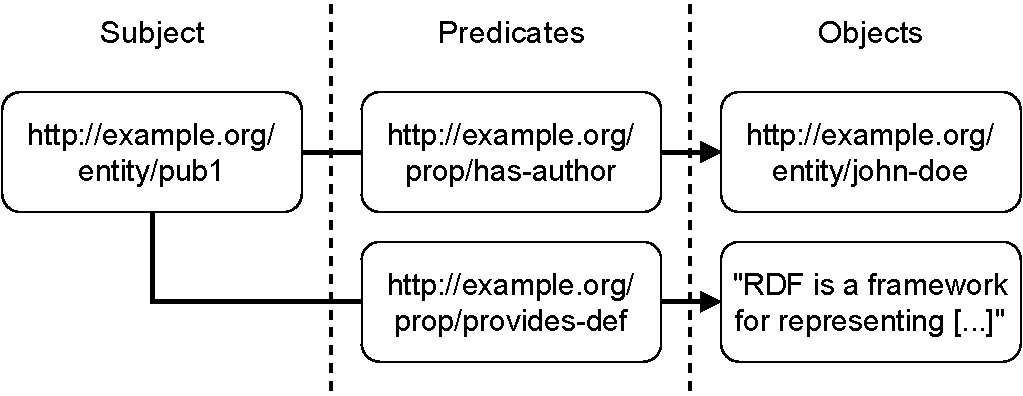
\includegraphics[max width=0.7\columnwidth]{/tex/example-basic/figures/triple_example}
\caption{A simple exemplary knowledge graph consisting of two RDF triples. The upper triple provides contextual information, the lower triple contentual information of the publication \emph{{pub1}}. All non-literal triple members are identified using IRIs. (Figure and caption adopted from~\cite{Martin21}.)}
\label{fig:contentual-contextual0}
\end{figure}
% RDFtex Figure Import End% RDFtex Figure Import Start
\begin{figure}[htb!]
\centering
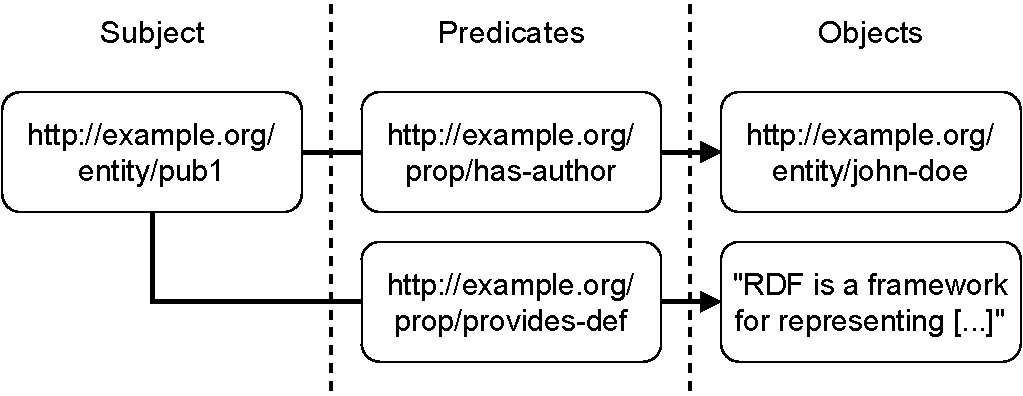
\includegraphics[max width=0.7\columnwidth]{/tex/example-basic/figures/triple_example}
\caption{A simple exemplary knowledge graph consisting of two RDF triples. The upper triple provides contextual information, the lower triple contentual information of the publication \emph{{pub1}}. All non-literal triple members are identified using IRIs. (Figure and caption adopted from~\cite{Martin21}.)}
\label{fig:contentual-contextual1}
\end{figure}
% RDFtex Figure Import End% RDFtex Figure Import Start
\begin{figure}[htb!]
\centering
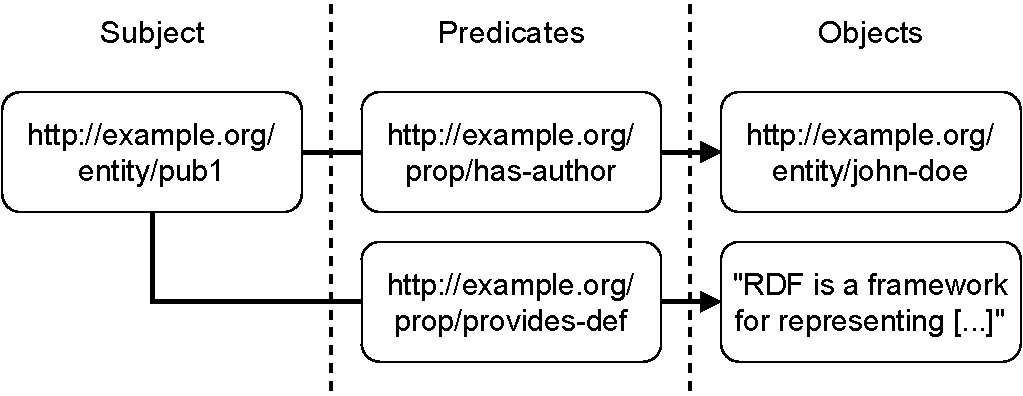
\includegraphics[max width=0.7\columnwidth]{/tex/example-basic/figures/triple_example}
\caption{A simple exemplary knowledge graph consisting of two RDF triples. The upper triple provides contextual information, the lower triple contentual information of the publication \emph{{pub1}}. All non-literal triple members are identified using IRIs. (Figure and caption adopted from~\cite{Martin21}.)}
\label{fig:contentual-contextual2}
\end{figure}
% RDFtex Figure Import End% RDFtex Figure Import Start
\begin{figure}[htb!]
\centering
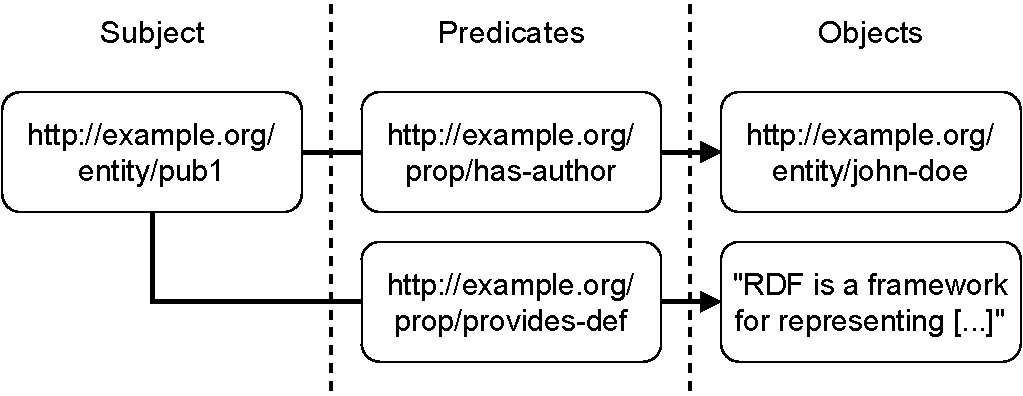
\includegraphics[max width=0.7\columnwidth]{/tex/example-basic/figures/triple_example}
\caption{A simple exemplary knowledge graph consisting of two RDF triples. The upper triple provides contextual information, the lower triple contentual information of the publication \emph{{pub1}}. All non-literal triple members are identified using IRIs. (Figure and caption adopted from~\cite{Martin21}.)}
\label{fig:contentual-contextual3}
\end{figure}
% RDFtex Figure Import End% RDFtex Figure Import Start
\begin{figure}[htb!]
\centering
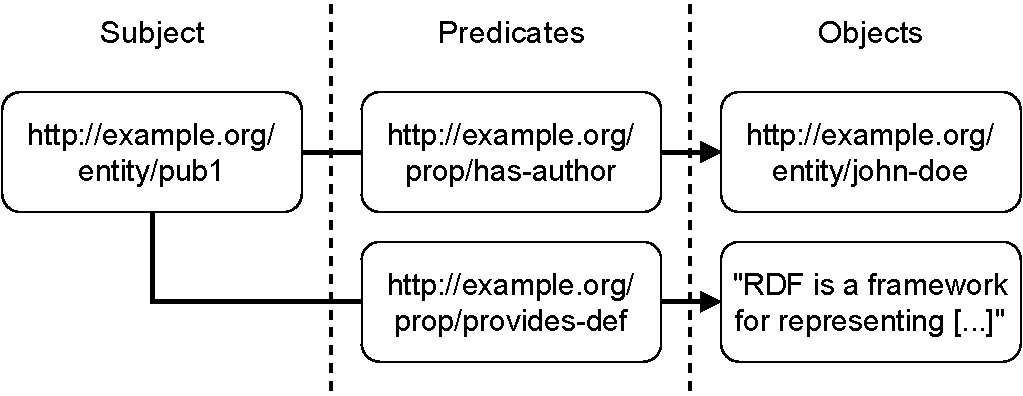
\includegraphics[max width=0.7\columnwidth]{/tex/example-basic/figures/triple_example}
\caption{A simple exemplary knowledge graph consisting of two RDF triples. The upper triple provides contextual information, the lower triple contentual information of the publication \emph{{pub1}}. All non-literal triple members are identified using IRIs. (Figure and caption adopted from~\cite{Martin21}.)}
\label{fig:contentual-contextual4}
\end{figure}
% RDFtex Figure Import End% RDFtex Figure Import Start
\begin{figure}[htb!]
\centering
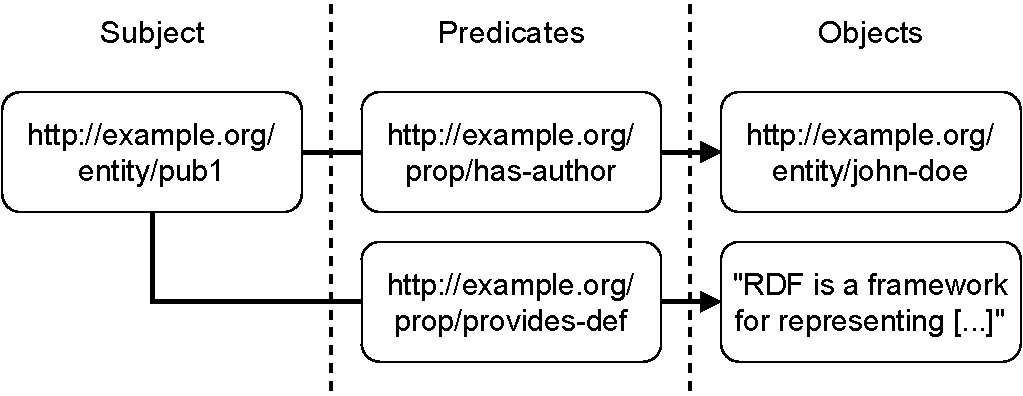
\includegraphics[max width=0.7\columnwidth]{/tex/example-basic/figures/triple_example}
\caption{A simple exemplary knowledge graph consisting of two RDF triples. The upper triple provides contextual information, the lower triple contentual information of the publication \emph{{pub1}}. All non-literal triple members are identified using IRIs. (Figure and caption adopted from~\cite{Martin21}.)}
\label{fig:contentual-contextual5}
\end{figure}
% RDFtex Figure Import End% RDFtex Figure Import Start
\begin{figure}[htb!]
\centering
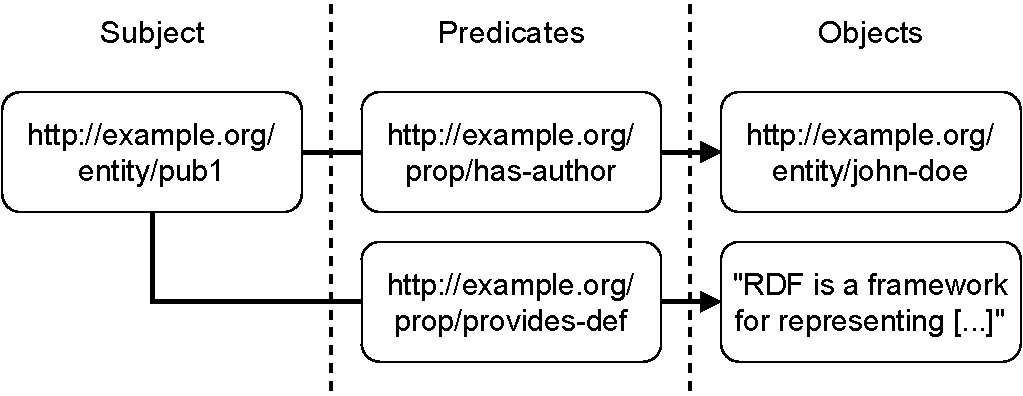
\includegraphics[max width=0.7\columnwidth]{/tex/example-basic/figures/triple_example}
\caption{A simple exemplary knowledge graph consisting of two RDF triples. The upper triple provides contextual information, the lower triple contentual information of the publication \emph{{pub1}}. All non-literal triple members are identified using IRIs. (Figure and caption adopted from~\cite{Martin21}.)}
\label{fig:contentual-contextual6}
\end{figure}
% RDFtex Figure Import End% RDFtex Figure Import Start
\begin{figure}[htb!]
\centering
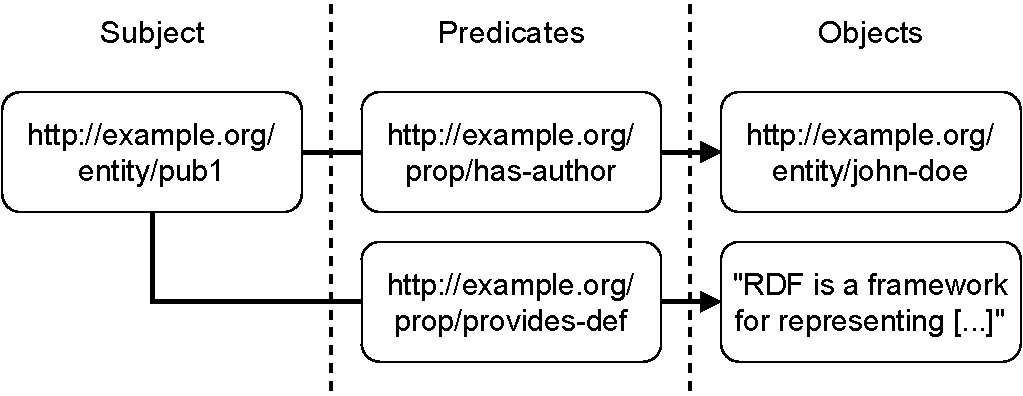
\includegraphics[max width=0.7\columnwidth]{/tex/example-basic/figures/triple_example}
\caption{A simple exemplary knowledge graph consisting of two RDF triples. The upper triple provides contextual information, the lower triple contentual information of the publication \emph{{pub1}}. All non-literal triple members are identified using IRIs. (Figure and caption adopted from~\cite{Martin21}.)}
\label{fig:contentual-contextual7}
\end{figure}
% RDFtex Figure Import End% RDFtex Figure Import Start
\begin{figure}[htb!]
\centering
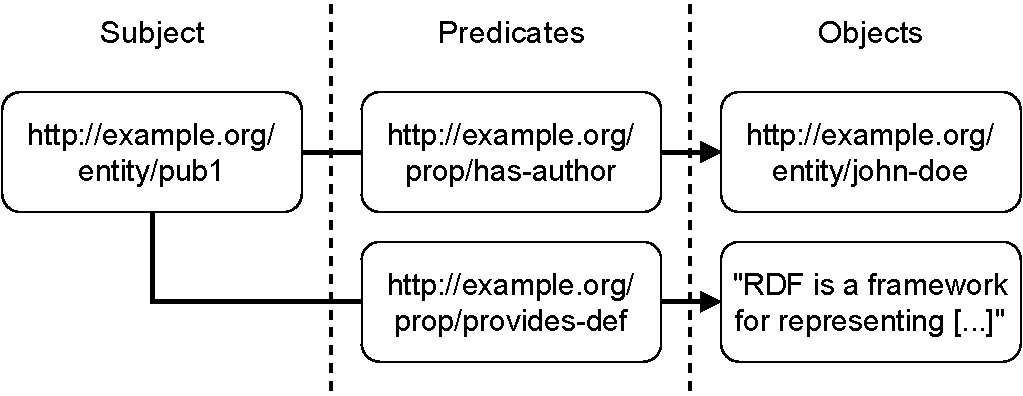
\includegraphics[max width=0.7\columnwidth]{/tex/example-basic/figures/triple_example}
\caption{A simple exemplary knowledge graph consisting of two RDF triples. The upper triple provides contextual information, the lower triple contentual information of the publication \emph{{pub1}}. All non-literal triple members are identified using IRIs. (Figure and caption adopted from~\cite{Martin21}.)}
\label{fig:contentual-contextual8}
\end{figure}
% RDFtex Figure Import End% RDFtex Figure Import Start
\begin{figure}[htb!]
\centering
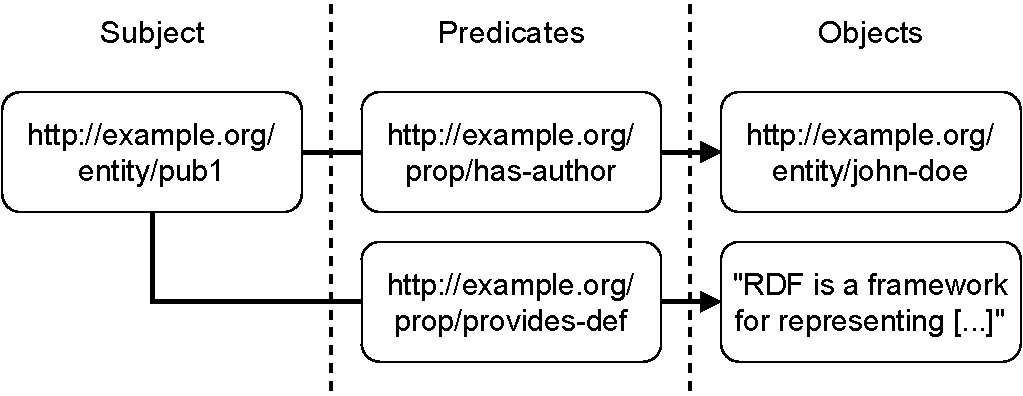
\includegraphics[max width=0.7\columnwidth]{/tex/example-basic/figures/triple_example}
\caption{A simple exemplary knowledge graph consisting of two RDF triples. The upper triple provides contextual information, the lower triple contentual information of the publication \emph{{pub1}}. All non-literal triple members are identified using IRIs. (Figure and caption adopted from~\cite{Martin21}.)}
\label{fig:contentual-contextual9}
\end{figure}
% RDFtex Figure Import End% RDFtex Figure Import Start
\begin{figure}[htb!]
\centering
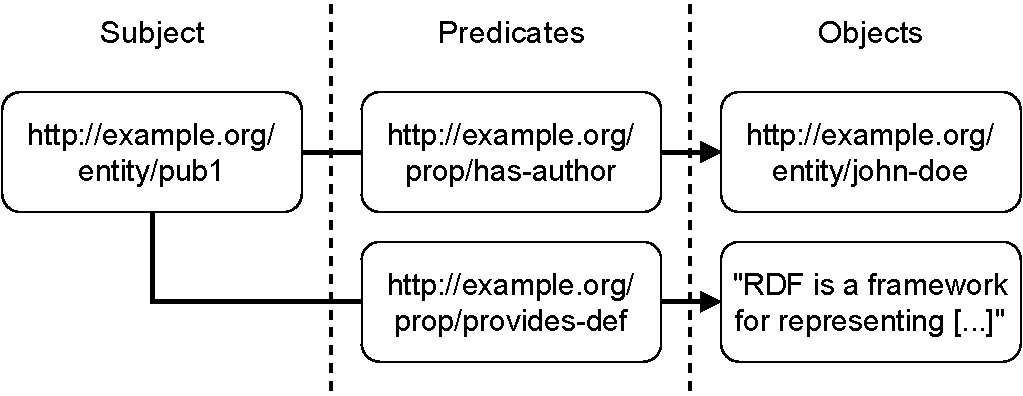
\includegraphics[max width=0.7\columnwidth]{/tex/example-basic/figures/triple_example}
\caption{A simple exemplary knowledge graph consisting of two RDF triples. The upper triple provides contextual information, the lower triple contentual information of the publication \emph{{pub1}}. All non-literal triple members are identified using IRIs. (Figure and caption adopted from~\cite{Martin21}.)}
\label{fig:contentual-contextual10}
\end{figure}
% RDFtex Figure Import End% RDFtex Figure Import Start
\begin{figure}[htb!]
\centering
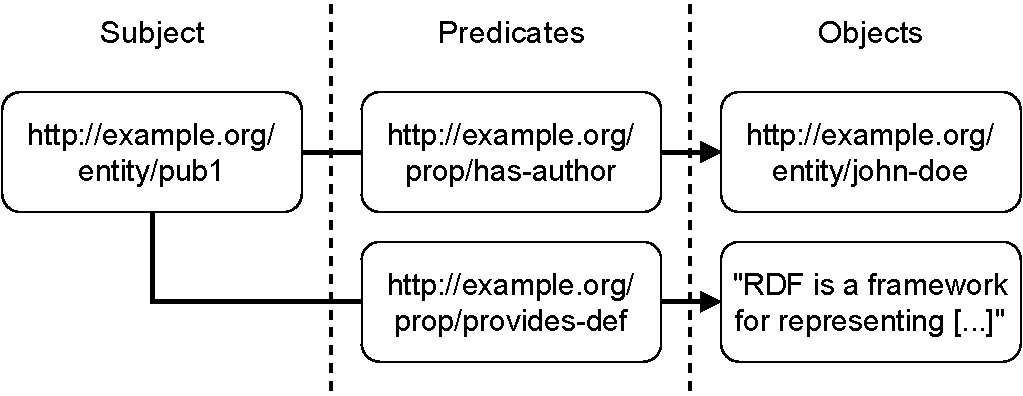
\includegraphics[max width=0.7\columnwidth]{/tex/example-basic/figures/triple_example}
\caption{A simple exemplary knowledge graph consisting of two RDF triples. The upper triple provides contextual information, the lower triple contentual information of the publication \emph{{pub1}}. All non-literal triple members are identified using IRIs. (Figure and caption adopted from~\cite{Martin21}.)}
\label{fig:contentual-contextual11}
\end{figure}
% RDFtex Figure Import End% RDFtex Figure Import Start
\begin{figure}[htb!]
\centering
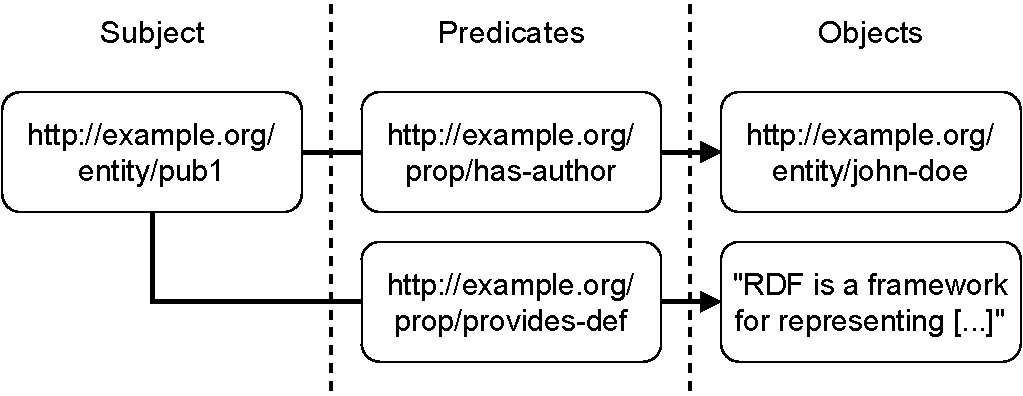
\includegraphics[max width=0.7\columnwidth]{/tex/example-basic/figures/triple_example}
\caption{A simple exemplary knowledge graph consisting of two RDF triples. The upper triple provides contextual information, the lower triple contentual information of the publication \emph{{pub1}}. All non-literal triple members are identified using IRIs. (Figure and caption adopted from~\cite{Martin21}.)}
\label{fig:contentual-contextual12}
\end{figure}
% RDFtex Figure Import End% RDFtex Figure Import Start
\begin{figure}[htb!]
\centering
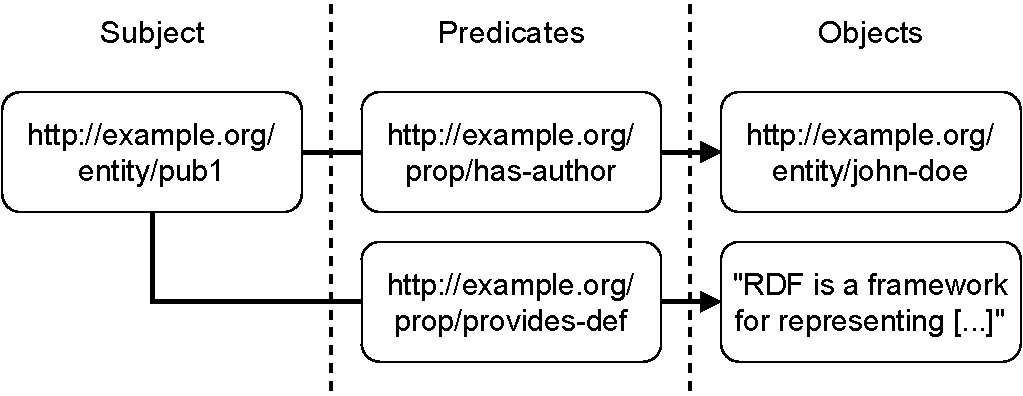
\includegraphics[max width=0.7\columnwidth]{/tex/example-basic/figures/triple_example}
\caption{A simple exemplary knowledge graph consisting of two RDF triples. The upper triple provides contextual information, the lower triple contentual information of the publication \emph{{pub1}}. All non-literal triple members are identified using IRIs. (Figure and caption adopted from~\cite{Martin21}.)}
\label{fig:contentual-contextual13}
\end{figure}
% RDFtex Figure Import End% RDFtex Figure Import Start
\begin{figure}[htb!]
\centering
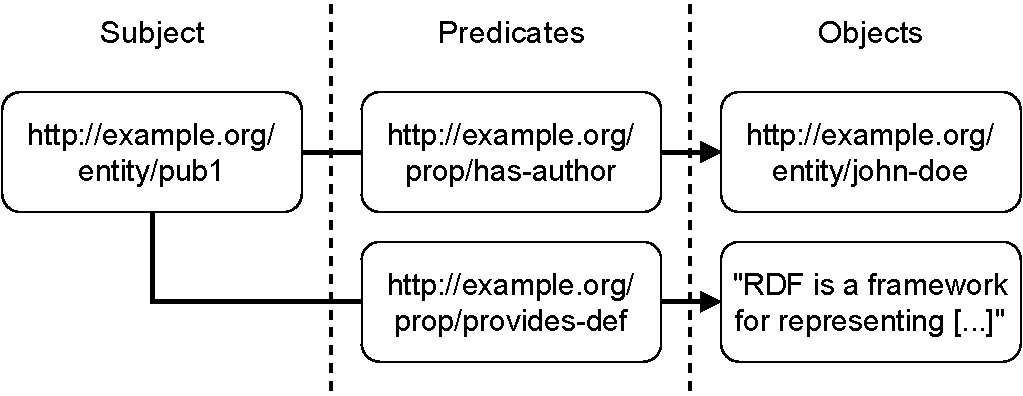
\includegraphics[max width=0.7\columnwidth]{/tex/example-basic/figures/triple_example}
\caption{A simple exemplary knowledge graph consisting of two RDF triples. The upper triple provides contextual information, the lower triple contentual information of the publication \emph{{pub1}}. All non-literal triple members are identified using IRIs. (Figure and caption adopted from~\cite{Martin21}.)}
\label{fig:contentual-contextual14}
\end{figure}
% RDFtex Figure Import End% RDFtex Figure Import Start
\begin{figure}[htb!]
\centering
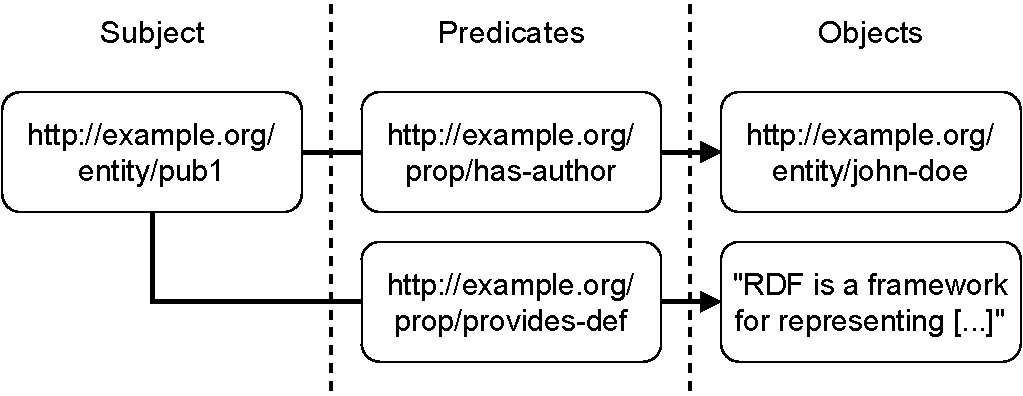
\includegraphics[max width=0.7\columnwidth]{/tex/example-basic/figures/triple_example}
\caption{A simple exemplary knowledge graph consisting of two RDF triples. The upper triple provides contextual information, the lower triple contentual information of the publication \emph{{pub1}}. All non-literal triple members are identified using IRIs. (Figure and caption adopted from~\cite{Martin21}.)}
\label{fig:contentual-contextual15}
\end{figure}
% RDFtex Figure Import End% RDFtex Figure Import Start
\begin{figure}[htb!]
\centering
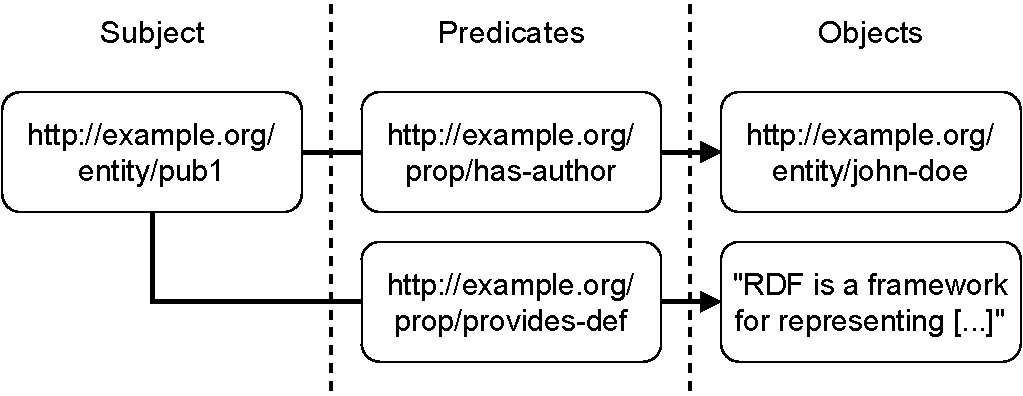
\includegraphics[max width=0.7\columnwidth]{/tex/example-basic/figures/triple_example}
\caption{A simple exemplary knowledge graph consisting of two RDF triples. The upper triple provides contextual information, the lower triple contentual information of the publication \emph{{pub1}}. All non-literal triple members are identified using IRIs. (Figure and caption adopted from~\cite{Martin21}.)}
\label{fig:contentual-contextual16}
\end{figure}
% RDFtex Figure Import End% RDFtex Figure Import Start
\begin{figure}[htb!]
\centering
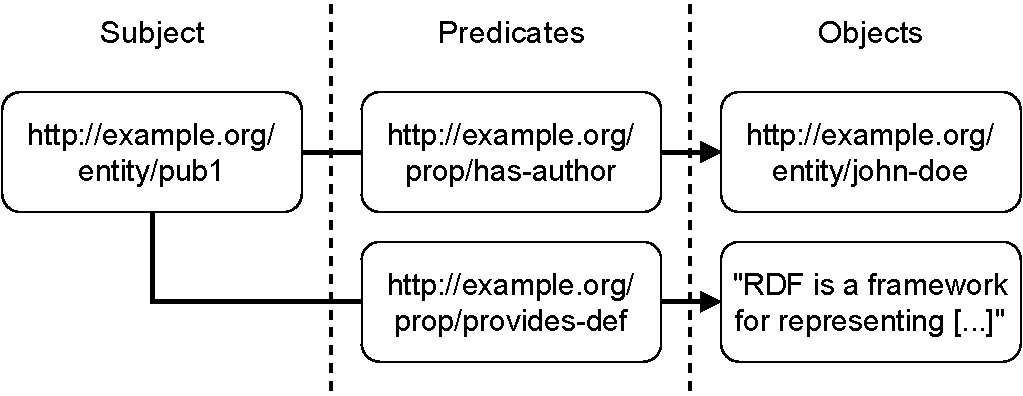
\includegraphics[max width=0.7\columnwidth]{/tex/example-basic/figures/triple_example}
\caption{A simple exemplary knowledge graph consisting of two RDF triples. The upper triple provides contextual information, the lower triple contentual information of the publication \emph{{pub1}}. All non-literal triple members are identified using IRIs. (Figure and caption adopted from~\cite{Martin21}.)}
\label{fig:contentual-contextual17}
\end{figure}
% RDFtex Figure Import End% RDFtex Figure Import Start
\begin{figure}[htb!]
\centering
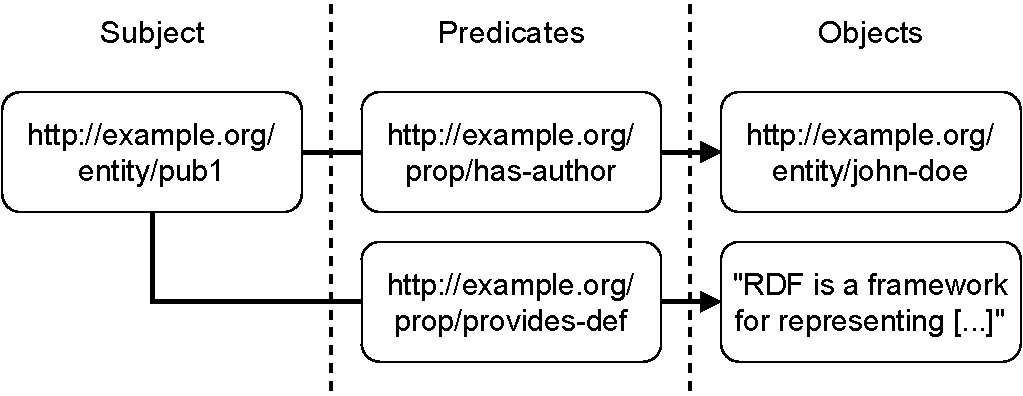
\includegraphics[max width=0.7\columnwidth]{/tex/example-basic/figures/triple_example}
\caption{A simple exemplary knowledge graph consisting of two RDF triples. The upper triple provides contextual information, the lower triple contentual information of the publication \emph{{pub1}}. All non-literal triple members are identified using IRIs. (Figure and caption adopted from~\cite{Martin21}.)}
\label{fig:contentual-contextual18}
\end{figure}
% RDFtex Figure Import End% RDFtex Figure Import Start
\begin{figure}[htb!]
\centering
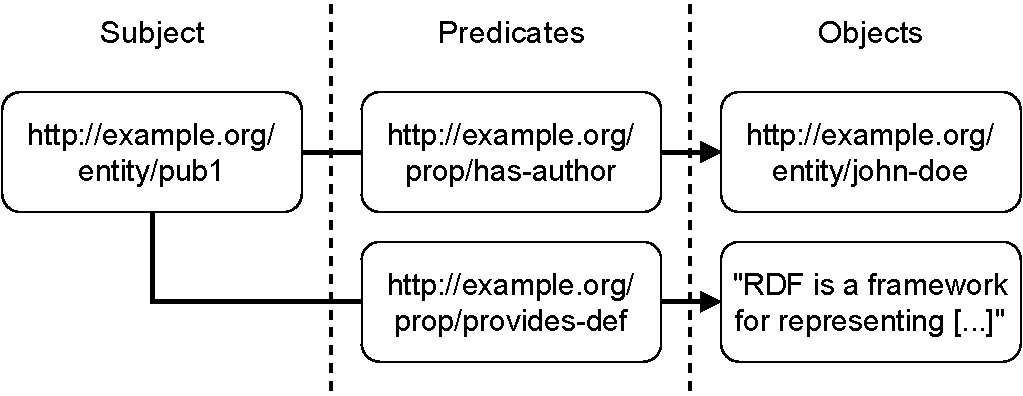
\includegraphics[max width=0.7\columnwidth]{/tex/example-basic/figures/triple_example}
\caption{A simple exemplary knowledge graph consisting of two RDF triples. The upper triple provides contextual information, the lower triple contentual information of the publication \emph{{pub1}}. All non-literal triple members are identified using IRIs. (Figure and caption adopted from~\cite{Martin21}.)}
\label{fig:contentual-contextual19}
\end{figure}
% RDFtex Figure Import End
\Cref{fig:contentual-contextual0} shows an imported figure.

\subsection{Software Import}

% RDFtex Software Import Start
\begin{software}
Prot{\'{e}}g{\'{e}}-2000~\cite{DBLP:conf/amia/NoyCFKTVM03}\\
Available at: \url{https://protege.stanford.edu}\\
Description: ``Prot\'{e}g\'{e}-2000 is an open-source tool that assists users in the construction of large electronic knowledge bases. It has an intuitive user interface that enables developers to create and edit domain ontologies."~\cite{DBLP:conf/amia/NoyCFKTVM03}
\label{software:protege0}
\end{software}
% RDFtex Software Import End% RDFtex Software Import Start
\begin{software}
Prot{\'{e}}g{\'{e}}-2000~\cite{DBLP:conf/amia/NoyCFKTVM03}\\
Available at: \url{https://protege.stanford.edu}\\
Description: ``Prot\'{e}g\'{e}-2000 is an open-source tool that assists users in the construction of large electronic knowledge bases. It has an intuitive user interface that enables developers to create and edit domain ontologies."~\cite{DBLP:conf/amia/NoyCFKTVM03}
\label{software:protege1}
\end{software}
% RDFtex Software Import End% RDFtex Software Import Start
\begin{software}
Prot{\'{e}}g{\'{e}}-2000~\cite{DBLP:conf/amia/NoyCFKTVM03}\\
Available at: \url{https://protege.stanford.edu}\\
Description: ``Prot\'{e}g\'{e}-2000 is an open-source tool that assists users in the construction of large electronic knowledge bases. It has an intuitive user interface that enables developers to create and edit domain ontologies."~\cite{DBLP:conf/amia/NoyCFKTVM03}
\label{software:protege2}
\end{software}
% RDFtex Software Import End% RDFtex Software Import Start
\begin{software}
Prot{\'{e}}g{\'{e}}-2000~\cite{DBLP:conf/amia/NoyCFKTVM03}\\
Available at: \url{https://protege.stanford.edu}\\
Description: ``Prot\'{e}g\'{e}-2000 is an open-source tool that assists users in the construction of large electronic knowledge bases. It has an intuitive user interface that enables developers to create and edit domain ontologies."~\cite{DBLP:conf/amia/NoyCFKTVM03}
\label{software:protege3}
\end{software}
% RDFtex Software Import End% RDFtex Software Import Start
\begin{software}
Prot{\'{e}}g{\'{e}}-2000~\cite{DBLP:conf/amia/NoyCFKTVM03}\\
Available at: \url{https://protege.stanford.edu}\\
Description: ``Prot\'{e}g\'{e}-2000 is an open-source tool that assists users in the construction of large electronic knowledge bases. It has an intuitive user interface that enables developers to create and edit domain ontologies."~\cite{DBLP:conf/amia/NoyCFKTVM03}
\label{software:protege4}
\end{software}
% RDFtex Software Import End% RDFtex Software Import Start
\begin{software}
Prot{\'{e}}g{\'{e}}-2000~\cite{DBLP:conf/amia/NoyCFKTVM03}\\
Available at: \url{https://protege.stanford.edu}\\
Description: ``Prot\'{e}g\'{e}-2000 is an open-source tool that assists users in the construction of large electronic knowledge bases. It has an intuitive user interface that enables developers to create and edit domain ontologies."~\cite{DBLP:conf/amia/NoyCFKTVM03}
\label{software:protege5}
\end{software}
% RDFtex Software Import End% RDFtex Software Import Start
\begin{software}
Prot{\'{e}}g{\'{e}}-2000~\cite{DBLP:conf/amia/NoyCFKTVM03}\\
Available at: \url{https://protege.stanford.edu}\\
Description: ``Prot\'{e}g\'{e}-2000 is an open-source tool that assists users in the construction of large electronic knowledge bases. It has an intuitive user interface that enables developers to create and edit domain ontologies."~\cite{DBLP:conf/amia/NoyCFKTVM03}
\label{software:protege6}
\end{software}
% RDFtex Software Import End% RDFtex Software Import Start
\begin{software}
Prot{\'{e}}g{\'{e}}-2000~\cite{DBLP:conf/amia/NoyCFKTVM03}\\
Available at: \url{https://protege.stanford.edu}\\
Description: ``Prot\'{e}g\'{e}-2000 is an open-source tool that assists users in the construction of large electronic knowledge bases. It has an intuitive user interface that enables developers to create and edit domain ontologies."~\cite{DBLP:conf/amia/NoyCFKTVM03}
\label{software:protege7}
\end{software}
% RDFtex Software Import End% RDFtex Software Import Start
\begin{software}
Prot{\'{e}}g{\'{e}}-2000~\cite{DBLP:conf/amia/NoyCFKTVM03}\\
Available at: \url{https://protege.stanford.edu}\\
Description: ``Prot\'{e}g\'{e}-2000 is an open-source tool that assists users in the construction of large electronic knowledge bases. It has an intuitive user interface that enables developers to create and edit domain ontologies."~\cite{DBLP:conf/amia/NoyCFKTVM03}
\label{software:protege8}
\end{software}
% RDFtex Software Import End% RDFtex Software Import Start
\begin{software}
Prot{\'{e}}g{\'{e}}-2000~\cite{DBLP:conf/amia/NoyCFKTVM03}\\
Available at: \url{https://protege.stanford.edu}\\
Description: ``Prot\'{e}g\'{e}-2000 is an open-source tool that assists users in the construction of large electronic knowledge bases. It has an intuitive user interface that enables developers to create and edit domain ontologies."~\cite{DBLP:conf/amia/NoyCFKTVM03}
\label{software:protege9}
\end{software}
% RDFtex Software Import End% RDFtex Software Import Start
\begin{software}
Prot{\'{e}}g{\'{e}}-2000~\cite{DBLP:conf/amia/NoyCFKTVM03}\\
Available at: \url{https://protege.stanford.edu}\\
Description: ``Prot\'{e}g\'{e}-2000 is an open-source tool that assists users in the construction of large electronic knowledge bases. It has an intuitive user interface that enables developers to create and edit domain ontologies."~\cite{DBLP:conf/amia/NoyCFKTVM03}
\label{software:protege10}
\end{software}
% RDFtex Software Import End% RDFtex Software Import Start
\begin{software}
Prot{\'{e}}g{\'{e}}-2000~\cite{DBLP:conf/amia/NoyCFKTVM03}\\
Available at: \url{https://protege.stanford.edu}\\
Description: ``Prot\'{e}g\'{e}-2000 is an open-source tool that assists users in the construction of large electronic knowledge bases. It has an intuitive user interface that enables developers to create and edit domain ontologies."~\cite{DBLP:conf/amia/NoyCFKTVM03}
\label{software:protege11}
\end{software}
% RDFtex Software Import End% RDFtex Software Import Start
\begin{software}
Prot{\'{e}}g{\'{e}}-2000~\cite{DBLP:conf/amia/NoyCFKTVM03}\\
Available at: \url{https://protege.stanford.edu}\\
Description: ``Prot\'{e}g\'{e}-2000 is an open-source tool that assists users in the construction of large electronic knowledge bases. It has an intuitive user interface that enables developers to create and edit domain ontologies."~\cite{DBLP:conf/amia/NoyCFKTVM03}
\label{software:protege12}
\end{software}
% RDFtex Software Import End% RDFtex Software Import Start
\begin{software}
Prot{\'{e}}g{\'{e}}-2000~\cite{DBLP:conf/amia/NoyCFKTVM03}\\
Available at: \url{https://protege.stanford.edu}\\
Description: ``Prot\'{e}g\'{e}-2000 is an open-source tool that assists users in the construction of large electronic knowledge bases. It has an intuitive user interface that enables developers to create and edit domain ontologies."~\cite{DBLP:conf/amia/NoyCFKTVM03}
\label{software:protege13}
\end{software}
% RDFtex Software Import End% RDFtex Software Import Start
\begin{software}
Prot{\'{e}}g{\'{e}}-2000~\cite{DBLP:conf/amia/NoyCFKTVM03}\\
Available at: \url{https://protege.stanford.edu}\\
Description: ``Prot\'{e}g\'{e}-2000 is an open-source tool that assists users in the construction of large electronic knowledge bases. It has an intuitive user interface that enables developers to create and edit domain ontologies."~\cite{DBLP:conf/amia/NoyCFKTVM03}
\label{software:protege14}
\end{software}
% RDFtex Software Import End% RDFtex Software Import Start
\begin{software}
Prot{\'{e}}g{\'{e}}-2000~\cite{DBLP:conf/amia/NoyCFKTVM03}\\
Available at: \url{https://protege.stanford.edu}\\
Description: ``Prot\'{e}g\'{e}-2000 is an open-source tool that assists users in the construction of large electronic knowledge bases. It has an intuitive user interface that enables developers to create and edit domain ontologies."~\cite{DBLP:conf/amia/NoyCFKTVM03}
\label{software:protege15}
\end{software}
% RDFtex Software Import End% RDFtex Software Import Start
\begin{software}
Prot{\'{e}}g{\'{e}}-2000~\cite{DBLP:conf/amia/NoyCFKTVM03}\\
Available at: \url{https://protege.stanford.edu}\\
Description: ``Prot\'{e}g\'{e}-2000 is an open-source tool that assists users in the construction of large electronic knowledge bases. It has an intuitive user interface that enables developers to create and edit domain ontologies."~\cite{DBLP:conf/amia/NoyCFKTVM03}
\label{software:protege16}
\end{software}
% RDFtex Software Import End% RDFtex Software Import Start
\begin{software}
Prot{\'{e}}g{\'{e}}-2000~\cite{DBLP:conf/amia/NoyCFKTVM03}\\
Available at: \url{https://protege.stanford.edu}\\
Description: ``Prot\'{e}g\'{e}-2000 is an open-source tool that assists users in the construction of large electronic knowledge bases. It has an intuitive user interface that enables developers to create and edit domain ontologies."~\cite{DBLP:conf/amia/NoyCFKTVM03}
\label{software:protege17}
\end{software}
% RDFtex Software Import End% RDFtex Software Import Start
\begin{software}
Prot{\'{e}}g{\'{e}}-2000~\cite{DBLP:conf/amia/NoyCFKTVM03}\\
Available at: \url{https://protege.stanford.edu}\\
Description: ``Prot\'{e}g\'{e}-2000 is an open-source tool that assists users in the construction of large electronic knowledge bases. It has an intuitive user interface that enables developers to create and edit domain ontologies."~\cite{DBLP:conf/amia/NoyCFKTVM03}
\label{software:protege18}
\end{software}
% RDFtex Software Import End% RDFtex Software Import Start
\begin{software}
Prot{\'{e}}g{\'{e}}-2000~\cite{DBLP:conf/amia/NoyCFKTVM03}\\
Available at: \url{https://protege.stanford.edu}\\
Description: ``Prot\'{e}g\'{e}-2000 is an open-source tool that assists users in the construction of large electronic knowledge bases. It has an intuitive user interface that enables developers to create and edit domain ontologies."~\cite{DBLP:conf/amia/NoyCFKTVM03}
\label{software:protege19}
\end{software}
% RDFtex Software Import End
\Cref{software:protege0} shows an imported software.


